



\documentclass[10pt,a4paper]{article}

% ─── Packages ─────────────────────────────────────────
\usepackage{fontspec}
\setmainfont{Times New Roman}

\usepackage[top=1.1cm,bottom=1.1cm,left=1.55cm,right=1.55cm]{geometry}
\usepackage{titlesec}
\usepackage{enumitem}
\usepackage{hyperref}
\usepackage{xcolor}
\usepackage{tabularx}
\usepackage{graphicx}
\usepackage{parskip}

% ─── Colors ───────────────────────────────────────────
\definecolor{primary}{RGB}{30,40,90}
\definecolor{namecolor}{RGB}{0,120,180}
\definecolor{accent}{RGB}{50,90,150}
\definecolor{rulecol}{RGB}{200,205,220}
\definecolor{gray}{RGB}{90,90,90}

\hypersetup{
    colorlinks=true,
    urlcolor=accent
}

\pagestyle{empty}
\setlength{\parskip}{0pt}

% ─── Section ──────────────────────────────────────────
\titleformat{\section}
    {\normalsize\bfseries\color{primary}}
    {}
    {0em}
    {}
    [\vspace{1pt}\textcolor{rulecol}{\titlerule[0.6pt]}\vspace{1pt}]

\titlespacing{\section}{0pt}{5pt}{2pt}

% ─── Entry ────────────────────────────────────────────
\newcommand{\entry}[3]{%
    \noindent
    \begin{tabularx}{\linewidth}{X r}
        \textbf{\color{primary}#1} &
        {\scriptsize\color{gray}#2}
    \end{tabularx}\\[-2pt]
    {\scriptsize\textit{\color{gray}#3}}
    \vspace{1pt}
}

% ─── Compact list ─────────────────────────────────────
\newenvironment{cvitems}{
    \begin{itemize}[
        leftmargin=1.15em,
        topsep=0pt,
        itemsep=0.5pt,
        parsep=0pt,
        partopsep=0pt
    ]
}{
    \end{itemize}
}

% ═════════════════════════════════════════════════════
\begin{document}
% ─── HEADER ───────────────────────────────────────────

\noindent
\begin{tabularx}{\linewidth}{@{}X r@{}}

% ─── Thông tin bên trái ───
\begin{minipage}[c]{\linewidth}
    {\LARGE\bfseries\color{namecolor} Hồ Huỳnh Nhu}\\[2pt]

    {\large\bfseries\color{primary}
    Nhân Viên IT}\\[3pt]

    {\scriptsize\color{gray}
    20/10/2003
    \enspace\textcolor{rulecol}{|}
    \enspace (+84) 367 503 477
    \enspace\textcolor{rulecol}{|}
    \enspace
    \href{mailto:hhnhu2003@gmail.com}{hhnhu2003@gmail.com}
    \enspace\textcolor{rulecol}{|}
    \enspace TP. Hồ Chí Minh}\\[2pt]

    {\scriptsize
    \href{https://github.com/hohuynhnhu}
    {https://github.com/hohuynhnhu}
    \enspace\textcolor{rulecol}{|}
    \enspace
    \href{https://www.facebook.com/huynhnhu.ho.961}
    {https://www.facebook.com/huynhnhu.ho.961}
}
\end{minipage}

&
% ─── Avatar bên phải ───
\begin{minipage}[c]{2.2cm}
    \raggedleft
    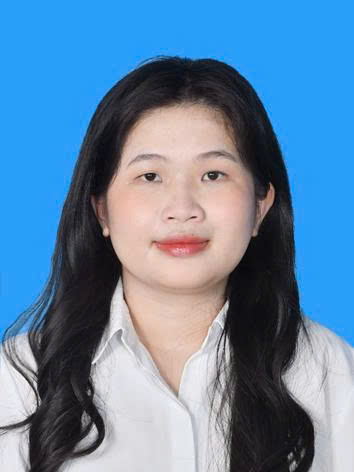
\includegraphics[
        width=2.2cm,
        height=2.7cm,
        keepaspectratio
    ]{assets/avt.jpg}
\end{minipage}

\end{tabularx}

\vspace{3pt}

\textcolor{rulecol}{\rule{\linewidth}{0.6pt}}

% ─── MỤC TIÊU ─────────────────────────────────────────

\section*{Mục Tiêu Nghề Nghiệp}

{\small
Sinh viên Công nghệ Thông tin năm cuối, định hướng phát triển trong lĩnh vực
IT và Backend Python. Có kinh nghiệm triển khai, vận hành và tích hợp
hệ thống phần mềm, cơ sở dữ liệu, API và các dịch vụ nội bộ. Có khả năng
xử lý sự cố, tự động hóa công việc bằng Python và hỗ trợ người dùng trong
quá trình sử dụng phần mềm. Đồng thời có kinh nghiệm về AI/ML, Data Engineering
và xây dựng dashboard phục vụ vận hành.
}

% ─── HỌC VẤN ──────────────────────────────────────────

\section*{Học Vấn}

\entry
{Trường Đại học Giao thông Vận tải TP.HCM (UTH)}
{10/2022 -- Dự kiến 10/2026}
{Cử nhân Công nghệ Thông tin -- Đã hoàn thành chương trình học}

{\small
\begin{cvitems}
    \item GPA: 3.4 / 4.0
    \enspace|\enspace
    \textbf{Học bổng Xuất sắc} -- HK1 năm 2025
    \item \textbf{Giải Nhì -- Track AI}
    \enspace Hội nghị Nghiên cứu Khoa học Sinh viên UTH 2025
\end{cvitems}
}

% ─── KỸ NĂNG ──────────────────────────────────────────

\section*{Kỹ Năng Kỹ Thuật}

{\small
\begin{tabularx}{\linewidth}{@{}lX@{}}

\textbf{IT \& Hệ thống}
&
Windows, xử lý sự cố phần mềm/phần cứng cơ bản,
cấu hình hệ thống, giám sát dịch vụ, hỗ trợ người dùng

\\[1.5pt]

\textbf{Backend \& API}
&
Python, FastAPI, Node.js, NestJS, RESTful API,
tích hợp và kết nối các hệ thống

\\[1.5pt]

\textbf{Cơ sở dữ liệu}
&
PostgreSQL, SQL Server, MongoDB, Firebase,
Supabase, truy vấn và quản lý dữ liệu

\\[1.5pt]

\textbf{Data \& Automation}
&
Python Script, dbt, Airflow, xử lý dữ liệu,
tự động hóa quy trình và báo cáo

\\[1.5pt]

\textbf{AI / ML}
&
Machine Learning, Deep Learning, CNN, YOLO,
Siamese Network, Transformer

\\[1.5pt]

\textbf{Web \& Mobile}
&
Nuxt.js, Vue 3, TypeScript, Flutter, Kotlin

\\[1.5pt]

\textbf{Công cụ}
&
Git, Docker, Postman, VS Code, Android Studio,
Figma, Power BI, Jira, Confluence
\\[1.5pt]

\textbf{Tin học văn phòng}
&
Thành thạo Microsoft Office

\\[1.5pt]

\textbf{Tiếng Anh}
&
Đọc hiểu tài liệu kỹ thuật; giao tiếp chuyên môn cơ bản

\end{tabularx}
}

% ─── KINH NGHIỆM ──────────────────────────────────────

\section*{Kinh Nghiệm Làm Việc}

\entry
{Gotik Consulting -- Data Engineer}
{Python \textbar{} dbt \textbar{} PostgreSQL \textbar{} Airflow \textbar{} Power BI}
{03/2026 -- 05/2026}

{\small
\begin{cvitems}

    \item Thu thập và xử lý dữ liệu nghiệp vụ từ hệ thống
    Odoo phục vụ phân tích và báo cáo.

    \item Xây dựng pipeline dữ liệu bằng Python + dbt,
    lưu trữ trên Neon PostgreSQL.

    \item Thiết lập Apache Airflow tự động chạy và
    giám sát pipeline theo chu kỳ hàng giờ.

    \item Kết nối Power BI để xây dựng dashboard
    theo dõi các chỉ số hoạt động.

\end{cvitems}
}

% ─── DỰ ÁN ────────────────────────────────────────────

\section*{Dự Án Nổi Bật}

% ─── FALL DETECTION ───────────────────────────────────
% ─── FALL DETECTION ───────────────────────────────────

\entry
{Fall Detection -- Hệ Thống Phát Hiện Té Ngã}
{Python \textbar{} FastAPI \textbar{} YOLOv8 Pose \textbar{} MediaPipe \textbar{} Transformer}
{2025}

{\small
\begin{cvitems}

    \item Xây dựng hệ thống phân tích hành vi người và phát hiện té ngã
    thời gian thực, kết hợp Rule-based và AI Transformer.

    \item Phát triển backend/API và pipeline AI, sử dụng
   MediaPipe + YOLOv8 Pose và sliding window
    30 frames $\times$ 200 features.

    \item Đạt 97.8\% Mean Accuracy, tích hợp
    Mobile App và Web Admin để quản lý và nhận cảnh báo.

    \item GitHub:
    \href{https://github.com/hohuynhnhu/Fall-Detection}
    {github.com/hohuynhnhu/Fall-Detection}

\end{cvitems}
}

\vspace{3pt}

% ─── VEHICLESCAN ──────────────────────────────────────

\entry
{VehicleScan -- Hệ Thống Bãi Xe Thông Minh IoT \& AI}
{Python \textbar{} YOLO \textbar{} CNN \textbar{} Siamese \textbar{} ESP32 \textbar{} Firebase}
{03/2025 -- 03/2026}

{\small
\begin{cvitems}

    \item Thu thập, làm sạch và xây dựng dataset phục vụ
    huấn luyện các mô hình AI nhận diện phương tiện.

    \item Huấn luyện và đánh giá CNN, YOLO, Siamese Network;
    xây dựng Rule-based kết hợp AI và dữ liệu cảm biến.

    \item Tích hợp AI, IoT và ứng dụng thông qua
    API/Firebase; đạt Giải Nhì -- Track AI,
    Hội nghị Nghiên cứu Khoa học Sinh viên UTH 2025.
    \item GitHub:
    \href{https://github.com/LeKhang-cn22h/VehicleScanner.git}
    {github.com/LeKhang-cn22h/VehicleScanner.git}
\end{cvitems}
}

% ─── THÔNG TIN THÊM ──────────────────────────────────

\section*{Thông Tin Thêm}

{\small
\begin{tabularx}{\linewidth}{@{}lX@{}}

\textbf{Kỹ năng mềm}
&
Giải quyết vấn đề \textbar{} Ham học hỏi \textbar{}
Chủ động xử lý sự cố \textbar{} Chịu áp lực tốt

\\[2pt]

\textbf{Khác}
&
Có khả năng hỗ trợ người dùng, hướng dẫn sử dụng phần mềm,
đào tạo người dùng không chuyên và phối hợp xử lý sự cố hệ thống.

\\[2pt]

\textbf{Thời gian}
&
Sẵn sàng làm việc theo ca và linh hoạt theo yêu cầu công việc.

\end{tabularx}
}

\end{document}